\documentclass{cugrep}

\usepackage{pdfpages}
\title{中国地质大学研究生课程论文\TeX{}模板}
\classname{\TeX{}模板教程}
\college{计算机学院}
\major{计算机科学与技术}
\sno{20131001333}
\teacher{某某某}
\class{硕士}
\author{Timozer}
\begin{document}

\maketitle

\frontmatter
\cugabstract{
    这是中国地质大学(武汉)研究生课程论文的 \LaTeX{}模板的说明文档. 
    主要对模板进行了介绍, 安装, 使用等方面的说明, 此外还写了模板开发
    过程的日志, 可以通过它来了解每一版中实现了哪些功能.
}
\cugkeywords{\TeX{}, \LaTeX{}, 模板, 报告}
\makeabstract 

\tableofcontents
\listoffigures
\listoftables
\clearpage

\mainmatter
\chapter{介绍}
\section{简介}
这份中国地质大学(武汉)研究生课程论文的 \LaTeX{} 模板是我根据中国地大学(武汉)
研究生课程论文的 {\sc Word} 版来编写的. 值得一提的是, 在 {\sc Word} 版中只
定义了封面的内容和下一页的评语表, 对其他格式并没有明确的要求, 因此, 在这份 \LaTeX{} 
模板中有关其他方面的格式都是没有标准可以参照的, 一切以我的审美为标准~:)~.

在此之前我好像并没有看到有人写过地大的 \TeX{} 课程论文模板. 因此, 鄙人在此斗胆献丑 (抱拳). 
才疏学浅, 难免有许多纰漏, 还望各位能够指出, 我会真心承认错误并积极改进~\verb|^_^|~.

本模板的编码参考了很多其他大学的 \TeX{} 论文模板, 在此表示感谢. 目前仍然在开发中, 虽
然用其写一个文档已经不成问题了, 但是还缺乏各种各样的让人用起来很舒服的功能. 因此, 希望
有 ``牛人'' 可以添加新功能或是对本模板进行除错.

\section{开发目标}
本模板旨在推广 \TeX{} 这一优秀排版软件在地大的应用, 为广大同学提供一个方便, 美观的
课程报告模板, 减少写报告时候因格式问题而带来的麻烦. 

本模板的目标是将模板做成开箱即用的形式. 我看了一些模板, 都有很多参数需要作者自己设置, 然而许多
文档作者并不需要或者是并不知道这些设置. 作为一个模板, 他们只是希望, 拿到就可以使用, {\sc Word}
模板需要自己设置参数吗? 不需要. 而且很多模板只是提供了封面及页面的格式, 标题的样式等等. 至于
在写作过程中的一些特殊输入需求, 还是得作者自己解决问题. 我想的是, 可以为作者提供一个友好
的写作环境, 至于那些杂七杂八的东西, 模版提供了支持, 不需要作者自己操心. 我会为这个目标而努力.

\section{\TeX{} Logos 测试}
\TeX{}, \LaTeX{}, \LaTeXe{}, \XeTeX{}, \XeLaTeX{}, \LuaTeX{}, \LuaLaTeX{}, 

\MF{}, \MP{}, \BIBTEX, \AMSTEX

除了 \texttt{\textbackslash MP} 命令, 其他的我都定义了小写形式, 以方便输入.
当然这样做可能会和其他一些宏包 (我不知道有哪些) 的命令冲突, 如果你在使用的过程中发现冲突了, 
请给我提供反馈, 我好及时纠正, 不胜感激. 

\texttt{\textbackslash MP} 命令, 即 \MP{} Logo, 之所以没有定义小写形式, 主要是因为 
\texttt{\textbackslash mp} 是个数学符号 $\mp$ .

\section{软件环境}
本模板在开发的时候是使用 MacOS + Texlive2017 的环境. 在该系统环境下可以正常编译文档.

如果你使用 Linux 系统, 我想也不会存在不能使用的问题. 

因为我本人是使用命令行来编译文档, 所以请不要问我 TeXMaker, TeXWorks, TeXShop 等等软件如何配置编译参数,
我不会. 你们可以自行在互联网上搜索. 具体的参数啦, 或是编译步骤啦, 请参考本模板中的 \texttt{Makefile}
文件. 
\subsection{MacOS \& Linux}
如果你使用的是 MacOS 或者是 Linux 系统, 那么请安装 Texlive2017, 至于你使用什么编辑器编辑源文档, 那全看你
个人的喜好. 该模板使用的编译系统是 \xelatex. 我推荐你使用完全安装, 这样你就不会有这样那样的错误.

\subsection{Windows}
Windows 系统的情况我不清楚, 但是我想也一样, 你可以安装 Texlive2017 或者以上版本来试着编译文档,
看能否行得通. 编译的时候请设置好编译参数, 具体设置自行搜索答案. 
\chapter{使用方法}
\section{安装}
本模板并不需要安装, 你可以在模板目录下写自己的报告文档, 也可以直接修改 demo.tex 文档 
(当然我肯定不建议你这样做, 因为这个文档的内容可以在你以后需要的时候回来查看. 呸, 其实
主要是因为这个文档是我写得啦, 尊重一下我好吧).

以下对本模板中的文件做一个说明: 
\begin{table}[htbp]
    \caption{模板文件说明}
    \label{tab:clsfiles}
    \begin{tabular*}{\textwidth}{>{\small \ttfamily \centering}p{.3\linewidth}>{\small}p{.63\linewidth}}
    \toprule
    文件名 & 文件说明 \\
    \midrule
    cugrep.cls & 这是本模板的文档类, 在使用模板的时候需要在导言区引入, \tcodeinline{tex}{\documentclass{cugrep}} ; \\
    timozercode.sty & 这是为方便代码引入而写的一个 code 宏包, 主要用于代码和伪代码的插入; \\
    timozerfont.sty & 这个文件用于文档中的字体设置, 中英文字体分开设置, 并且提供了从初号到小五的字体大小命令; \\
    timozertexlogos.sty & 这是宏包主要引入了提供 \TeX{} logos 的宏包; \\
    timozerbib.sty & 对参考文献的格式做了一个设置; \\
    timozerdirtree.sty & 目录树; \\
    demo.tex & 本说明文档的 tex 源码文件; \\
    README.md & 本项目的说明文档; \\
    Makefile & make 程序使用的文件; \\
    LICENSE & 本项目的协议; \\
    pyglangs.txt & 代码支持的语言类型; \\
    pygstyles.txt & 代码高亮支持的风格.  \\
    \bottomrule
\end{tabular*}
\end{table}
\section{建立自己的文档}

在开始写你的文档之前, 你的目录应该是这个样子:

\begin{forest}
    pic dir tree,
    pic root,
    for tree={%
        dir,
    },
    [{/.} 
        [cugrep.cls, file] 
        [demo.pdf, file] 
        [demo.tex, file] 
        [LICENSE, file] 
        [Makefile, file]
        [pyglangs.txt, file] 
        [pygstyles.txt, file] 
        [README.md, file] 
        [timozerbib.sty, file] 
        [timozercode.sty, file] 
        [timozerdirtree.sty, file]
        [timozerfont.sty, file]
        [timozertexlogos.sty, file]
    ]
\end{forest}

接下来新建一个 \texttt{tex} 文档, 假如是 \texttt{rep.tex}. 当然你可以直接修改
\texttt{demo.tex} 文件, 将自己内容添加进去. 但是我不建议你这样做.

\section{添加封面信息}
我提供的模板是一个文档类, 不仅仅是一个宏包. 因此, 在你的报告开头应该引入模板类, 向下面这样:
\begin{minted}{tex}
    \documentclass{cugrep}
\end{minted}

请注意, 目前这个版本中不需要提供任何参数.

接下来需要你为报告提供一些基本信息, 比如说课程报告的标题, 该课程的名字,
你所在的学院以及专业, 还有你的学号, 老师的名字, 你的类别 (本科生, 硕士,
博士, 还是进修生等), 你的名字.

像本文档这样:
\begin{minted}[firstnumber=3]{tex}
    \title{中国地质大学研究生课程论文\TeX{}模板}
    \classname{\TeX{}模板教程}
    \college{计算机学院}
    \major{计算机科学与技术}
    \sno{20131001333}
    \teacher{某某某}
    \class{硕士}
    \author{Timozer}
\end{minted}

然后通过 \tcodeinline{tex}{\maketitle} 命令来制作封面以及评语表. 

\section{文档结构}

每一篇报告的格式基本都是类似的. 前面的是封面和评语表, 接着就是摘要, 紧接着
是各种目录等. 而摘要和目录等在 \TeX{} 里面称之为 \texttt{frontmatter}. 

摘要和目录之后就是正文了, 也就是 \texttt{mainmatter}.

我看了一些论文的模板, 大都是将附录放在了致谢和参考文献等的后面. 因此, 在正文
之后, 我们需要没有章节号的致谢和参考文献. 这属于 \texttt{backmatter}.

如果你想添加附录, 那么以 \texttt{appendix} 开始, 开启章节号, 然后添加附录章节.

因此, 最后你的文档结构是这样子的:
\begin{minted}{tex}
    \begin{document}
        \maketitle

        \frontmatter
        \makeabstract
        \tableofcontents
        \clearpage

        \mainmatter
        \chapter{正文章节}

        \backmatter
        \chapter{致谢}

        \appendix
        \chapter{附录}
    \end{document}
\end{minted}

请注意 \texttt{frontmatter, mainmatter, backmatter, appendix} 等的顺序, 不要
随意使用, 否则, 可能得不到你想要的结果. 关于具体的含义, 请参看表\ref{tab:mattersdiff}.
\begin{table}[htpb]
    \centering
    \caption{\small \texttt{frontmatter, mainmatter, backmatter, appendix} 的区别}
    \label{tab:mattersdiff}
    \begin{tabular*}{\textwidth}{>{\small \ttfamily}p{.2\textwidth} >{\small}p{.75\textwidth}}
        \toprule
        项目 & 功能 \\
        \midrule
        frontmatter & 关闭 Chapter 计数, 页码使用 Roman 形式. 请注意, 关闭 Chapter 计数不是指将 Chapter 计数归零, 而是直接就不使用该计数器. \\
        mainmatter & 打开 Chapter 计数, 使用 arabic 形式的页码. \\
        backmatter & 关闭 Chapter 计数, 页码形式不变. \\
        appendix & 打开 Chapter 计数, 并且使用 Alph 形式, 页码形式不变. \\
        \bottomrule
    \end{tabular*}
\end{table}

\section{生成文档}
当你写完你的文档的时候, 你就可以通过 \ttword{xelatex} 程序来编译生成 pdf 文档了.

如果你有 \texttt{make} 等工具的使用知识, 可以修改 \texttt{Makefile} 文件来简化
输入命令.

如果你不熟悉的话, 可以直接使用命令 \tcodeinline{sh}{$xelatex rep.tex} 来编译, 
当然, 这是在你没有添加参考文献的时候, 这样就能得到你的文档了. 如果你引用了参考
文献, 还需要 \texttt{bibtex} 来编译生成的 \texttt{aux} 文件, 比如这样:
\tcodeinline{sh}{$bibtex rep.aux}, 然后你还需要执行两次 
\tcodeinline{sh}{$xelatex rep.tex}.

整个的执行过程如下:
\begin{minted}{sh}
    $ xelatex rep.tex
    $ bibtex rep.aux
    $ xelatex rep.tex
    $ xelatex rep.tex
\end{minted}
最后生成的文档, 请参看附录~\ref{chapter:egdoc}~.

\section{参考文献类型}
文献类型: 
\begin{table}[htpb]
    \centering
    \caption{参考文献格式}
    \label{tab:bibformat}
    \begin{tabular*}{\textwidth}{>{\small\bfseries}p{.18\textwidth}>{\small}p{.36\textwidth}>{\small}p{.36\textwidth}}
        \toprule 
        文献类型 & 必须项目 & 可选项目 \\
        \midrule 
        article & author, title, journal, year & volume, number, pages, month, note \\
        book & author/editor, title, publisher, year & volume/number, series, address, edition, month, note \\
        booklet & title & author, howpublished, address, month, year, note \\
        inbook & author/editor, title, chapter/pages, publisher, year & volume/number, series, type, address, edition, month, note \\
        incollection & author, title, booktitle, publisher, year & editor, volume/number, series, type, chapter, pages, address, edition, month, note \\
        inproceedings & authore, title, booktitle, year & editor, volume/number, series, pages, address, month, organization, publisher, note \\
        manual & title & author, organization, address, edition, month, year, note \\
        mastersthesis & author, title, school, year & type, address, month, note \\
        misc & none & author, title, howpublished, month, year, note \\
        phdthesis & author, title, school, year & type, address, month, note \\
        proceedings & title, year & editor, volume/number, series, address, month, organization, publisher, note \\
        techreport & author, title, institution, year & type, number, address, month, note \\
        unpublished & author, title, note & month, year \\
        \bottomrule 
    \end{tabular*}
\end{table}
\chapter{实现细节}
我个人感觉从一个\tex 使用者, 到一个\tex 模板开发者, 是一个非常难的过程.
一个原因, 资料不全, 相当的不全. 中途遇到很多问题, 中文资料没有, 还得使用蹩脚的英语
去搜英文资料 (或许我得考虑认真学习一下英语了). 

我是在本科时候自己随便乱搞的一个简陋模板的基础上进行开发的. 最开始想着, 这东西没什么内容,
就把自己在开发过程中的一些细节, 想法等写下来, 供自己以后回顾, 也供大家来参考. 但是,
写着写着, 就觉得开发一个\tex 模板需要的东西太多了, 这小小的一章根本放不下, 于是就有了将
这些实现细节写成博客文章发出来的想法, 因此, 具体的内容不会在这里写了.

如果我写了这些文章, 我会在这篇说明文档和 README.md 文档中更新状态的, 敬请关注.
\chapter{版本开发记录日志}

\section{Version 0.3}
\label{sec:version_0_3}
因为想不起版本0.1--~0.2做了哪些功能, 所以在此就不介绍了.

这个版本主要是实现了中国地质大学(武汉)研究生课程论文 Word 模板中的封面和后面的评语表.
\section{Version 0.4}
\label{sec:version_0_4}

目前在开发中, 暂时实现了摘要的添加. 因为这个\TeX{}模板主要 使用的是
ctexbook 文档类, 所以没有摘要这一环境, 暂时添加了摘要环境. 我不是太
想使用摘要这个环境, 使用环境意味着摘要和关键词的格式需要自己调, 这
很不舒服.

2018年 1月26日 星期五 21时50分38秒 CST

我新定义了一个命令\tcodeinline{tex}{\makeabstract}, 像\tcodeinline{tex}{\maketitle}一样, 可以
使用这个命令来生成摘要页面. 在使用之前, 你必须给变量\tcodeinline{tex}{\cugabstract, \cugkeywords} 
赋值. 也许我可以起更好听的名字:).

2018年 1月28日 星期日 17时01分20秒 CST

为了使行文方便, 我重新定义了\tcodeinline{tex}{\frontmatter, \mainmatter, \backmatter} 这四个命令. 

\begin{itemize}
    \item \tcodeinline{tex}{\frontmatter} 这个命令实现的功能是关闭 chapter 计数, 使用 roman 数字来标识页码;
    \item \tcodeinline{tex}{\mainmatter} 这个命令实现的功能是打开 chapter 计数, 使用 arabic 数字来标识页码;
    \item \tcodeinline{tex}{\backmatter} 这个命令实现的功能是关闭 chapter 计数.
\end{itemize}

折腾了一会儿页眉页脚, 包括首页页眉页脚. 但是成果比较感人, 首页之外的页面实现了页眉页脚的设置,
页眉左边为``中国地质大学(武汉)研究生课程论文'', 右边为节标题, 节标题的格式有点儿不好,需要改进.
另一个就是首页的页眉页脚设置好像有点儿问题, 只是让它在下面显示页码, 结果没有显示, 目前还不知道问题所在. 

2018年 1月29日 星期一 12时04分22秒 CST

今天终于查到了首页页脚没显示的问题. 在 \tcodeinline{tex}{\ctexset} 里面设置 \tcodeinline{tex}{chapter} 的时候设置了页
面的格式为 \tcodeinline{tex}{empty}, 把后面的设置冲掉了. 现在更改为 \tcodeinline{tex}{plain} 格式. 新的问题又来了, 首
页页眉会显示一条横线, 看着不舒服, 去掉吧. 

ctex 本身对 appendix 的设置就很不错了, 所以我这里就不对其重新定义了, 删除了原来对 \tcodeinline{tex}{\appendix}
的重定义. 

看了好多大学的论文模板, 发现附录一般都是放在最后的, 而参考文献, 致谢这些在附录的前面. 这就产生了一个问题.
在写文档的时候, 我们用 \tcodeinline{tex}{\appendix} 命令来重置 chapter 计数, 并使用字母来表示章号, 而使用
 \tcodeinline{tex}{\backmatter} 来关闭 chapter 计数, 从而使 \tcodeinline{tex}{\chapter} 命令
 产生的章标题(参考文献, 致谢等) 不包含章号. 这样无形中的一个顺序使得结果和自己所想甚远. 
 \tcodeinline{tex}{\backmatter} 命令关闭 chapter 计数, \tcodeinline{tex}{\appendix} 是不会打开的.
所以这里要重新定义 \tcodeinline{tex}{\appendix}, 使得它会打开 chapter 计数. 

0.4 版本开发搞一段落. 回顾一下该版本实现的功能:

\begin{itemize}
    \item 添加了摘要命令 \tcodeinline{tex}{\makeabstract}, 使得可以方便生成摘要;
    \item 定义了报告的写作顺序, \tcodeinline{tex}{\frontmatter, \mainmatter, \backmatter, \appendix}, 严格按照这个顺序来定义
        报告的结构, 如果不按此来写, 很有可能不是你想要的结果;
    \item 重定义了 \tcodeinline{tex}{\frontmatter, \mainmatter, \appendix} 等命令.
\end{itemize}

\section{Version 0.5}

2018年 1月30日 星期二 17时07分04秒 CST

今天正式开始开发 0.5 版本.

昨天在推送 0.4 版本后发现了一个问题, 字体配置有问题. 0.4 版本及之前的版本中, 字体配置是我
自己在网上下载的字体, 而且也并没有将其安装到系统中, 只是将其放到了一个文件夹中, 然后使用
fontspec 宏包中的 \tcodeinline{tex}{\defaultfontfeature}命令指定其路径. 这就造成了只能使用该路径下的
字体的问题. 关于如何添加多个路径以及把 \LaTeX{} 默认搜索路径添加进来的操作, 我不会. 谷歌了
很久都没有查到, 所以就放弃了, 如果你们谁知道如何解决这个问题, 烦请联系我, 不胜感激. 

在放弃了那个方法后, 我就使用了 \LaTeX{} 的默认搜索路径, 并且把自己要使用的字体安装到系统中.
这样, 我就可以在 \LaTeX{} 中使用了. 

这个问题解决后, 突然发现又有新问题出现了 (程序开发中解决一个 BUG 又产生了一堆新的 BUG 的即
视感有木有 \verb|>_<| ). 那就是英文字体中的加粗, 斜体, 小型大写字母命令不起作用了, 无衬线和等宽字体
的命令还能骑作用, 不是太清楚什么问题, 在寻找中.

关于这个问题, 我也是谷歌了很久的, 烦. 资料出奇的少.

最终找到一个类似的问题, 他的解决方案是去掉了一个宏包, 然后就可以了. 我首先被这个人的想法
惊到了, 突然想起以前看过一篇文章, 讲得是一个不懂电脑的电脑维修人员维修电脑的方法, 他的修电脑
方法和这个人类似, 也是将电脑的零件各种拔插, 本来的开不了机的电脑就可以开机了 (ps. 难道这种
方法是计算机领域的一大特色\verb|^_^|).

我决定采用他这种方法. 首先不加入任何宏包, 看这是不是 ctexbook 文档类本身的问题 (ps. 很明显是
我想多了, 人家那么多大神在维护, 怎么可能出这种问题). 显然不是, 我又想会不会是我自己写的 
timozerfont.sty 这个文件出了问题 (ps. 才疏学浅, 出问题在所难免). 在测试文档里引入了我的宏包, 
测试通过, 并没有问题. 那么就是我引入的宏包之间的冲突了. 目前在排除中 \ldots .

在我将以下这些宏包关闭后, 字体正常了.

\begin{itemize}
    \item \{amstext, amsmath, amssymb, amsfonts, mathrsfs, bm, mathtools, newtxtext, courier\}
    \item \{graphicx, subcaption\}
    \item \{longtable, makecell, tabu, booktabs\}
    \item \{natbib\}
    \item \{timozercode\}, 这个是我自己写的一个宏包, 用来方便输入代码的, 具体用法应该在该模板大体完善的时候会写.
\end{itemize}


接下来一组一组的去开启这些宏包, 使用排除法来找出产生冲突的宏包. 

很幸运, 在我开启第一组的时候就发现那几个命令工作不正常了. 后面三组不用看了.

使用二分法, 经过几次测试后, 发现是 newtxtext 的问题. 

我又对该宏包进行了单独测试, 发现其和 ctexbook 文档类并不冲突, 奇哉怪哉. 难道
是和我写的 timozerfont.sty 宏包有冲突? 经过测试, 确实是和该宏包冲突, 在没有
找到解决方法之前, 我先把 newtxtext 宏包禁用了. 

2018年 2月 1日 星期四 10时28分29秒 CST

经过昨天的一番思想斗争以及查阅资料, 看宏包的说明文档, 我终于决定使用 minted 宏包来代替 lstlistings 宏包
来实现代码插入.

在为代码添加背景色的时候, 发现 color 宏包不能正常使用, 换成了 xcolor 宏包. 

今天实现了行内代码命令的定义, 提供了一个代码浮动体环境,
并且对代码环境的外观进行了设置. 基本任务完成, 如果有空,
我会考虑添加从文件中导入代码的功能.

2018年 2月 2日 星期五 12时17分51秒 CST

昨天的代码环境有点儿小瑕疵, 就是不能自动换行, 今天修正这个纰漏.

0.5 版本开发告一段落, 在此对其做一个总结.

首先是字体配置的问题. 在开发前几个版本的时候没有注意到字体的问题, 主要是写文档的时候因为功能不多,
也就没怎么使用不同的字体, 这不, 一旦开始使用不同的字体时候问题就出来了. 主要的问题就是文档默认的
中英文字体看着并不是很舒服, 其次就是一些字体命令竟然失效了. 

文档默认的中英文字体在花费几个小时的比对后, 选出来了一些好看的并且是大部分文档都会采用的字体. 
关于命令失效的问题, 找到了原因, 通过去掉一个宏包的方法修复好了.

接下来就是添加对代码的支持了. 因为我本身就是计算机专业的, 在写报告时候肯定会或多或少的需要在文档中
展示一些代码, 这个时候就需要很方便, 而且不用我每次去查相关文档就能引入代码的方法了. 为此, 我基于
minted 宏包 (之前是 lstlistings) 重新写了一个简化的宏包 timozercode. 

该宏包提供了行内代码的输入方式, 和代码段落以及代码浮动体的舒服方式, 基本的设置已经配好了, 只需要
输入代码即可, 如果不满意我的设置, 可以自己去修改.

我们在写报告的时候不仅仅需要代码, 有时会需要实现对伪代码的排版, 这个功能在该版本里面有了一个基本的
设置, 你可以自己查看代码来找到使用的方法, 我还没有详细地去做这方面的工作, 下一版中应该会添加进来. 

之后又添加了 \TeX{} 系统的 logo 输入宏包, 该宏包主要就是预引入 \TeX{} logos 的宏包, 方便大家在输入
的时候不用关心其在哪个宏包里, 自己需要用到哪个宏包, 不用你操心, 我已经给你做了这个工作了,
没其他的作用,

最后就是将参考文献这个功能添加进来. 

这就是 0.5 版本中实现的所有功能. 敬请期待下一版~:)~.

\section{Version 0.6}
\label{sec:version_0_6}

2018年 2月 2日 星期五 21时01分41秒 CST

我试图为这个模板提供一些新的环境命令来方便我们输入内容, 比如说插图环境, 我想定义一个新的环境将
插图环境包进去, 然后提供两个参数, 用来做插图的标题和标签, 这个环境自动将标题和标签放在闭合环境
命令前面 (close stuff or end part), 很可惜, 我们并不能这么做, 具体原因我查到了, 如代码\ref{code:envclosestuffparams}所示.

\begin{tcodeenv}{为什么 newenvironment 的参数不能放在 close stuff 中}{code:envclosestuffparams}
    \begin{minted}{tex}
    \newenvironment{foo}[1]%
    { ... open stuff ... }
    { ... close stuff ... }

    % is defined internally as
    \def\foo#1{...}
    \def\endfoo{...}
    % the end part has been defined by no arguments
    \newenvironment{foo}[1]%
    {\def\fooNoI{#1} some code #1}
    {some code \fooNoI}
    \end{minted}
\end{tcodeenv}

通过使用 xparse 宏包, 解决了这个问题.

重定义了 \tcodeinline{tex}{\ref{label}} 命令.

2018年 2月 3日 星期六 14时07分28秒 CST

提供了一个新的环境 tdirtree, 可以用来做目录树. 在 timozerdirtree 宏包里.

今天略写了一下说明文档, 将基本的东西写了一下. 目前的状况自己还算满意, 但是自己清楚还有
很多事情没做. 最近烦了, 暂时不想开发了, 原本的打算在该版本中加入的伪代码功能也没有去做,
因此 0.6 版本开发到此结束. 下一个版本什么时候开发, 我也不知道, 应该是等我有空想起来这个事情吧.

说明文档目前也暂时写到这儿了, 我想会在以后的版本开发过程中逐步完善说明文档. 你如果想用
这个模板, 却不知道该怎么用, 可以来问我, 当然如果你的 \TeX{} 基础知识过关的话, 可以自己
查看我写的代码来获得相应的用法.

我的联系方式在附录\ref{chapter:egdoc}中的表\ref{tab:contact}找到.

\section{Version 0.7}
2018年 2月 3日 星期六 17时44分02秒 CST

暂停开发.
\backmatter{}
% 这里是参考文献
%\tbib{bibFileName}

\chapter{致谢}

\appendix
\chapter{文档示例}
\label{chapter:egdoc}

这里我将示例文档的内容插入进来, 以供大家查看.

\begin{table}[htpb]
    \centering
    \caption{联系方式}
    \label{tab:contact}
    \begin{tabular}{>{\sffamily}l>{\ttfamily\small}l}
        \toprule
        E-mail & zhenyuwang94@gmail.com \\
        QQ & 878592748 \\
        Github & https://github.com/Timozer \\
        \bottomrule 
    \end{tabular}
\end{table}

不管用何种方式联系我, 请注明 ``CUGTeX模板问题''.
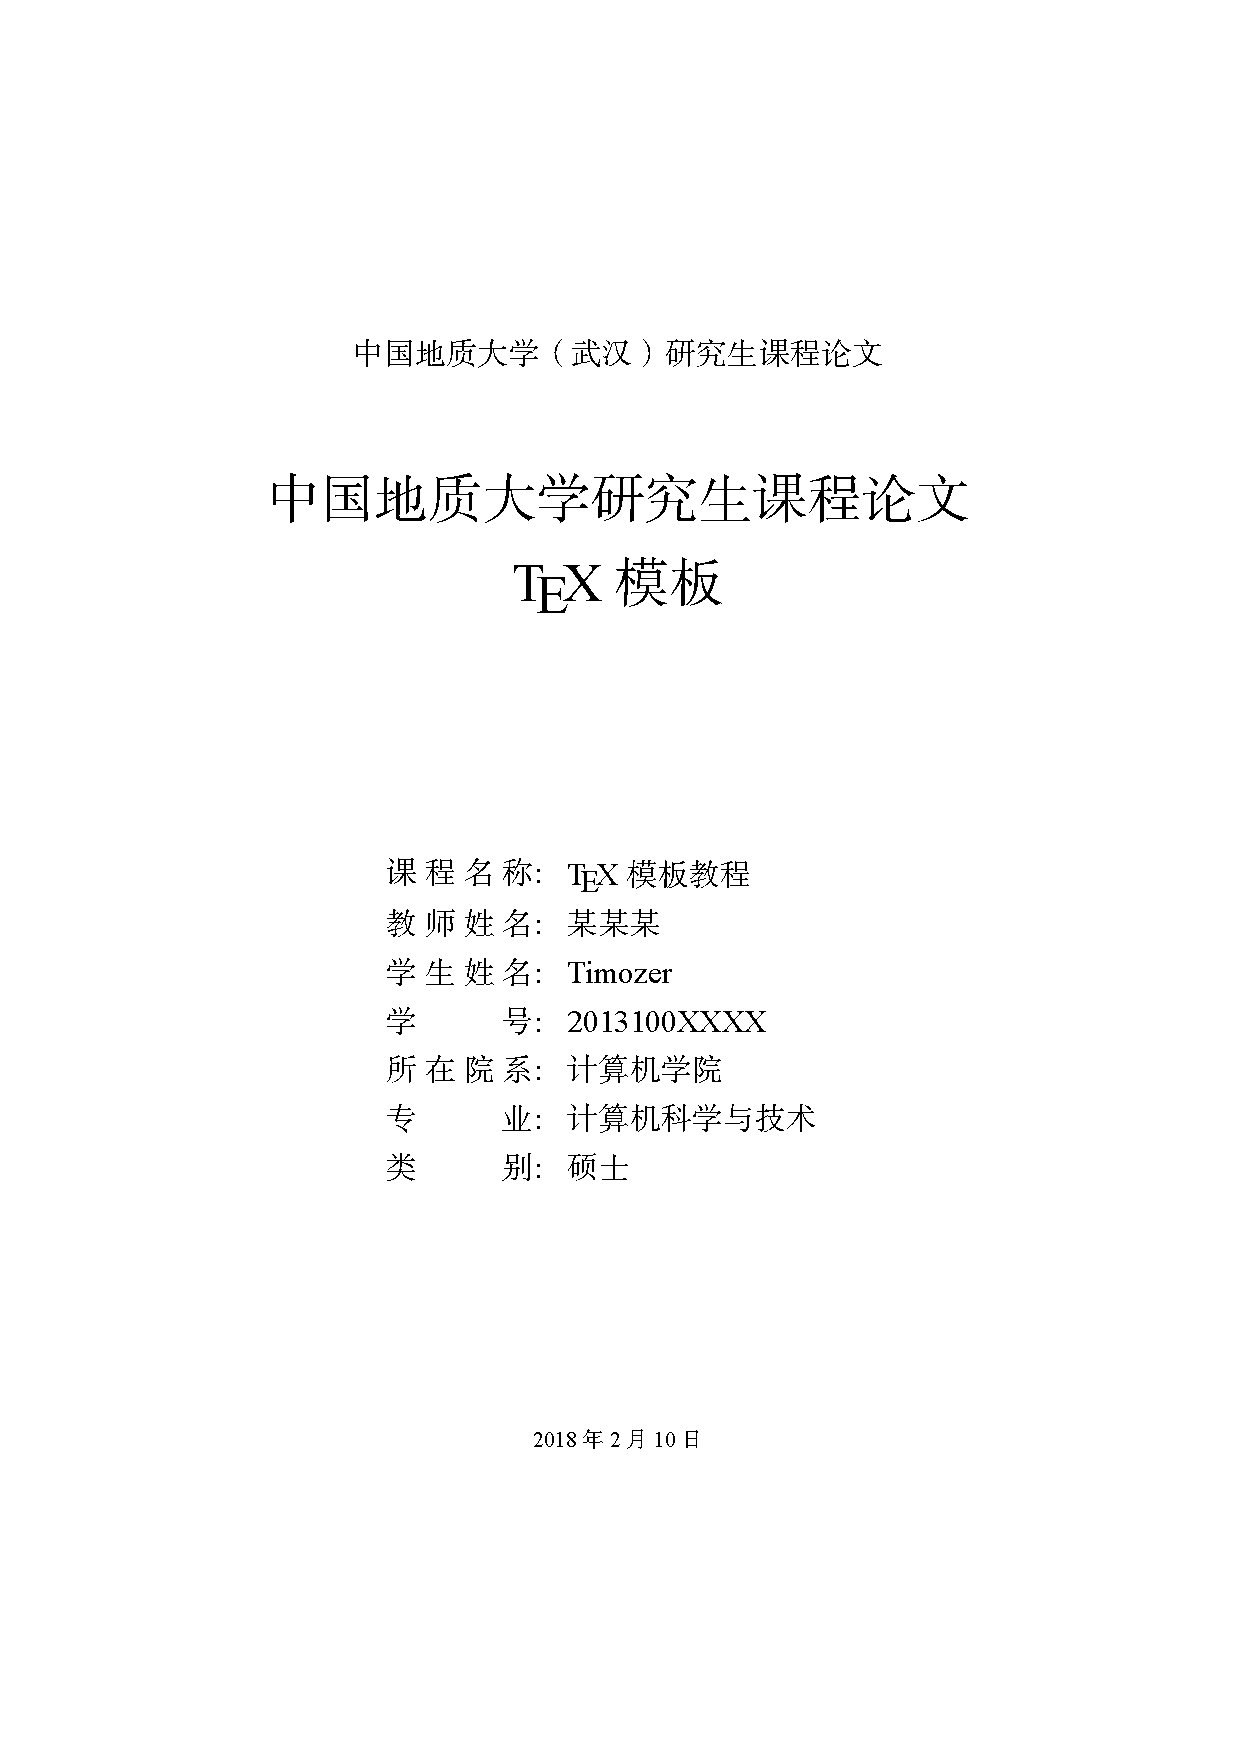
\includepdf[pages={1-4}, scale=0.9, pagecommand={\thispagestyle{empty}}, frame, nup=2x2]{example.pdf}
\includepdf[pages={5-7}, scale=0.9, pagecommand={\thispagestyle{empty}}, frame, nup=2x2]{example.pdf}

\chapter{LICENSE}
\cugrep 模板采用的是 GPLv3 协议, 下面给出简短说明, 详情请参看目录下的 LICENSE 文件.

Copyright © 2018 Timozer <zhenyuwang94@gmail.com>

This program is free software: you can redistribute it and/or modify
it under the terms of the GNU General Public License as published by
the Free Software Foundation, either version 3 of the License, or
(at your option) any later version.

This program is distributed in the hope that it will be useful,
but WITHOUT ANY WARRANTY; without even the implied warranty of
MERCHANTABILITY or FITNESS FOR A PARTICULAR PURPOSE.  See the
GNU General Public License for more details.

You should have received a copy of the GNU General Public License
along with this program.  If not, see <http://www.gnu.org/licenses/>.

%{\small \sffamily \input{LICENSE}}
\end{document}
